% Regenerate from this directory:
% latex -interaction=nonstopmode -halt-on-error garsia-wachs.tex
% dvisvgm --no-fonts --exact --bbox=papersize -o garsia-wachs.svg garsia-wachs.dvi
\documentclass[tikz,border=5pt]{standalone}
\usetikzlibrary{arrows.meta,backgrounds}
\pgfdeclarelayer{highlights}
\pgfsetlayers{highlights,background,main}
\definecolor{mergeblue}{RGB}{174,214,234}
\definecolor{nodeyellow}{RGB}{255,235,166}
\begin{document}
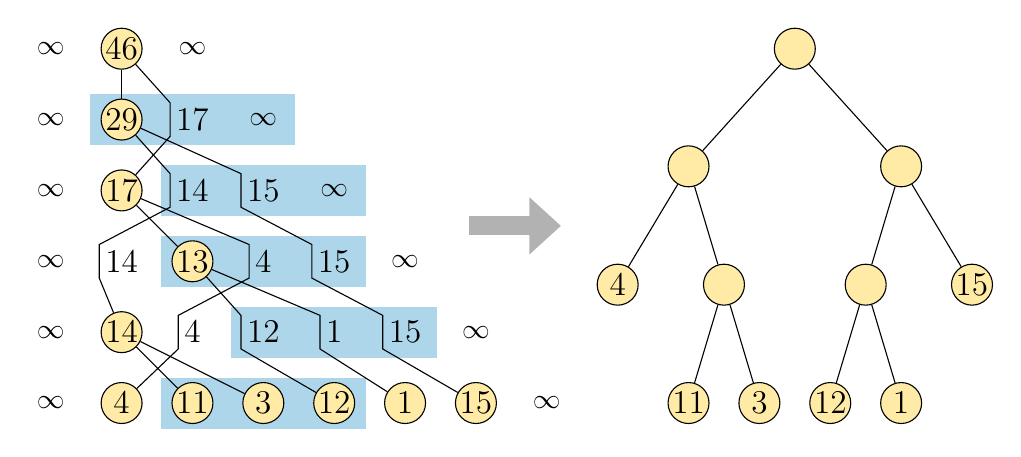
\begin{tikzpicture}[
  x=9mm,y=9mm,line width=.65pt,
  item/.style={inner sep=2pt,fill=white,font=\large},
  vertex/.style={circle,draw,fill=nodeyellow,inner sep=0pt,
    minimum size=5.2mm,font=\large}
]
  % The input is (4,11,3,12,1,15), with sum 46.
  % Read the merge history upward. Blue boxes select the next triple
  % (x,y,z) with x<=z. The first two entries merge, and their sum moves
  % left past smaller entries. Plain numbers track unchanged subtrees;
  % only the yellow circles are vertices of the phase-one tree.
  \begin{pgfonlayer}{highlights}
    \fill[mergeblue] (1.55,-.36) rectangle (4.45,.36);
    \fill[mergeblue] (2.55,.64) rectangle (5.45,1.36);
    \fill[mergeblue] (1.55,1.64) rectangle (4.45,2.36);
    \fill[mergeblue] (1.55,2.64) rectangle (4.45,3.36);
    \fill[mergeblue] (.55,3.64) rectangle (3.45,4.36);
  \end{pgfonlayer}

  % The forest after each merge, from bottom (row 0) to top (row 5).
  \foreach \id/\x/\weight in {a/1/4,b/2/11,c/3/3,d/4/12,e/5/1,f/6/15}
    \node[vertex] (r0\id) at (\x,0) {$\weight$};
  \node[vertex] (r1g) at (1,1) {$14$};
  \foreach \id/\x/\weight in {a/2/4,d/3/12,e/4/1,f/5/15}
    \node[item,fill=none] (r1\id) at (\x,1) {$\weight$};
  \node[vertex] (r2h) at (2,2) {$13$};
  \foreach \id/\x/\weight in {g/1/14,a/3/4,f/4/15}
    \node[item,fill=none] (r2\id) at (\x,2) {$\weight$};
  \node[vertex] (r3i) at (1,3) {$17$};
  \foreach \id/\x/\weight in {g/2/14,f/3/15}
    \node[item,fill=none] (r3\id) at (\x,3) {$\weight$};
  \node[vertex] (r4j) at (1,4) {$29$};
  \node[item,fill=none] (r4i) at (2,4) {$17$};
  \node[vertex] (r5k) at (1,5) {$46$};

  \foreach \row/\right in {0/7,1/6,2/5,3/4,4/3,5/2} {
    \node at (0,\row) {$\infty$};
    \node at (\right,\row) {$\infty$};
  }
  \begin{scope}[on background layer]
    % Each edge joins two vertices, bypassing unchanged subtree labels.
    \draw (r1g) -- (r0b);
    \draw (r1g) -- (r0c);
    \draw (r2h) -- (r1d.north west) -- (r1d.south west) -- (r0d);
    \draw (r2h) -- (r1e.north west) -- (r1e.south west) -- (r0e);
    \draw (r3i) -- (r2h);
    \draw (r3i) -- (r2a.north west) -- (r2a.south west)
      -- (r1a.north west) -- (r1a.south west) -- (r0a);
    \draw (r4j) -- (r3g.north west) -- (r3g.south west)
      -- (r2g.north west) -- (r2g.south west) -- (r1g);
    \draw (r4j) -- (r3f.north west) -- (r3f.south west)
      -- (r2f.north west) -- (r2f.south west)
      -- (r1f.north west) -- (r1f.south west) -- (r0f);
    \draw (r5k) -- (r4j);
    \draw (r5k) -- (r4i.north west) -- (r4i.south west) -- (r3i);
  \end{scope}

  \draw[-{Triangle[length=4mm,width=7mm]},gray!60,line width=2.4mm]
    (5.9,2.5) -- (7.2,2.5);

  % Phase three restores the input leaf order while retaining every leaf's
  % phase-one depth: (2,3,3,3,3,2). Internal sums are deliberately omitted,
  % as in the original illustration.
  \node[vertex] (root) at (10.5,5) {};
  \node[vertex] (left) at (9,3.34) {};
  \node[vertex] (right) at (12,3.34) {};
  \node[vertex] (four) at (8,1.67) {$4$};
  \node[vertex] (leftpair) at (9.5,1.67) {};
  \node[vertex] (rightpair) at (11.5,1.67) {};
  \node[vertex] (fifteen) at (13,1.67) {$15$};
  \node[vertex] (eleven) at (9,0) {$11$};
  \node[vertex] (three) at (10,0) {$3$};
  \node[vertex] (twelve) at (11,0) {$12$};
  \node[vertex] (one) at (12,0) {$1$};
  \foreach \parent/\child in {
    root/left,root/right,left/four,left/leftpair,right/rightpair,right/fifteen,
    leftpair/eleven,leftpair/three,rightpair/twelve,rightpair/one}
    \draw (\parent) -- (\child);
\end{tikzpicture}
\end{document}
